% Options for packages loaded elsewhere
\PassOptionsToPackage{unicode}{hyperref}
\PassOptionsToPackage{hyphens}{url}
%


\PassOptionsToPackage{table}{xcolor}

\documentclass[
  10pt,
  letterpaper,
]{article}

\usepackage{amsmath,amssymb}
\usepackage{iftex}
\ifPDFTeX
  \usepackage[T1]{fontenc}
  \usepackage[utf8]{inputenc}
  \usepackage{textcomp} % provide euro and other symbols
\else % if luatex or xetex
  \usepackage{unicode-math}
  \defaultfontfeatures{Scale=MatchLowercase}
  \defaultfontfeatures[\rmfamily]{Ligatures=TeX,Scale=1}
\fi
\usepackage{lmodern}
\ifPDFTeX\else  
    % xetex/luatex font selection
\fi
% Use upquote if available, for straight quotes in verbatim environments
\IfFileExists{upquote.sty}{\usepackage{upquote}}{}
\IfFileExists{microtype.sty}{% use microtype if available
  \usepackage[]{microtype}
  \UseMicrotypeSet[protrusion]{basicmath} % disable protrusion for tt fonts
}{}
\makeatletter
\@ifundefined{KOMAClassName}{% if non-KOMA class
  \IfFileExists{parskip.sty}{%
    \usepackage{parskip}
  }{% else
    \setlength{\parindent}{0pt}
    \setlength{\parskip}{6pt plus 2pt minus 1pt}}
}{% if KOMA class
  \KOMAoptions{parskip=half}}
\makeatother
\usepackage{xcolor}
\usepackage[top=0.85in,left=2.75in,footskip=0.75in]{geometry}
\setlength{\emergencystretch}{3em} % prevent overfull lines
\setcounter{secnumdepth}{-\maxdimen} % remove section numbering


\providecommand{\tightlist}{%
  \setlength{\itemsep}{0pt}\setlength{\parskip}{0pt}}\usepackage{longtable,booktabs,array}
\usepackage{calc} % for calculating minipage widths
% Correct order of tables after \paragraph or \subparagraph
\usepackage{etoolbox}
\makeatletter
\patchcmd\longtable{\par}{\if@noskipsec\mbox{}\fi\par}{}{}
\makeatother
% Allow footnotes in longtable head/foot
\IfFileExists{footnotehyper.sty}{\usepackage{footnotehyper}}{\usepackage{footnote}}
\makesavenoteenv{longtable}
\usepackage{graphicx}
\makeatletter
\def\maxwidth{\ifdim\Gin@nat@width>\linewidth\linewidth\else\Gin@nat@width\fi}
\def\maxheight{\ifdim\Gin@nat@height>\textheight\textheight\else\Gin@nat@height\fi}
\makeatother
% Scale images if necessary, so that they will not overflow the page
% margins by default, and it is still possible to overwrite the defaults
% using explicit options in \includegraphics[width, height, ...]{}
\setkeys{Gin}{width=\maxwidth,height=\maxheight,keepaspectratio}
% Set default figure placement to htbp
\makeatletter
\def\fps@figure{htbp}
\makeatother

% Use adjustwidth environment to exceed column width (see example table in text)
\usepackage{changepage}

% marvosym package for additional characters
\usepackage{marvosym}

% cite package, to clean up citations in the main text. Do not remove.
% Using natbib instead
% \usepackage{cite}

% Use nameref to cite supporting information files (see Supporting Information section for more info)
\usepackage{nameref,hyperref}

% line numbers
\usepackage[right]{lineno}

% ligatures disabled
\usepackage{microtype}
\DisableLigatures[f]{encoding = *, family = * }

% create "+" rule type for thick vertical lines
\newcolumntype{+}{!{\vrule width 2pt}}

% create \thickcline for thick horizontal lines of variable length
\newlength\savedwidth
\newcommand\thickcline[1]{%
  \noalign{\global\savedwidth\arrayrulewidth\global\arrayrulewidth 2pt}%
  \cline{#1}%
  \noalign{\vskip\arrayrulewidth}%
  \noalign{\global\arrayrulewidth\savedwidth}%
}

% \thickhline command for thick horizontal lines that span the table
\newcommand\thickhline{\noalign{\global\savedwidth\arrayrulewidth\global\arrayrulewidth 2pt}%
\hline
\noalign{\global\arrayrulewidth\savedwidth}}

% Text layout
\raggedright
\setlength{\parindent}{0.5cm}
\textwidth 5.25in 
\textheight 8.75in

% Bold the 'Figure #' in the caption and separate it from the title/caption with a period
% Captions will be left justified
\usepackage[aboveskip=1pt,labelfont=bf,labelsep=period,justification=raggedright,singlelinecheck=off]{caption}
\renewcommand{\figurename}{Fig}

% Remove brackets from numbering in List of References
\makeatletter
\renewcommand{\@biblabel}[1]{\quad#1.}
\makeatother

% Header and Footer with logo
\usepackage{lastpage,fancyhdr}
\usepackage{epstopdf}
%\pagestyle{myheadings}
\pagestyle{fancy}
\fancyhf{}
%\setlength{\headheight}{27.023pt}
%\lhead{\includegraphics[width=2.0in]{PLOS-submission.eps}}
\rfoot{\thepage/\pageref{LastPage}}
\renewcommand{\headrulewidth}{0pt}
\renewcommand{\footrule}{\hrule height 2pt \vspace{2mm}}
\fancyheadoffset[L]{2.25in}
\fancyfootoffset[L]{2.25in}
\lfoot{\today}
\makeatletter
\@ifpackageloaded{tcolorbox}{}{\usepackage[skins,breakable]{tcolorbox}}
\@ifpackageloaded{fontawesome5}{}{\usepackage{fontawesome5}}
\definecolor{quarto-callout-color}{HTML}{909090}
\definecolor{quarto-callout-note-color}{HTML}{0758E5}
\definecolor{quarto-callout-important-color}{HTML}{CC1914}
\definecolor{quarto-callout-warning-color}{HTML}{EB9113}
\definecolor{quarto-callout-tip-color}{HTML}{00A047}
\definecolor{quarto-callout-caution-color}{HTML}{FC5300}
\definecolor{quarto-callout-color-frame}{HTML}{acacac}
\definecolor{quarto-callout-note-color-frame}{HTML}{4582ec}
\definecolor{quarto-callout-important-color-frame}{HTML}{d9534f}
\definecolor{quarto-callout-warning-color-frame}{HTML}{f0ad4e}
\definecolor{quarto-callout-tip-color-frame}{HTML}{02b875}
\definecolor{quarto-callout-caution-color-frame}{HTML}{fd7e14}
\makeatother
\makeatletter
\@ifpackageloaded{caption}{}{\usepackage{caption}}
\AtBeginDocument{%
\ifdefined\contentsname
  \renewcommand*\contentsname{Table of contents}
\else
  \newcommand\contentsname{Table of contents}
\fi
\ifdefined\listfigurename
  \renewcommand*\listfigurename{List of Figures}
\else
  \newcommand\listfigurename{List of Figures}
\fi
\ifdefined\listtablename
  \renewcommand*\listtablename{List of Tables}
\else
  \newcommand\listtablename{List of Tables}
\fi
\ifdefined\figurename
  \renewcommand*\figurename{Figure}
\else
  \newcommand\figurename{Figure}
\fi
\ifdefined\tablename
  \renewcommand*\tablename{Table}
\else
  \newcommand\tablename{Table}
\fi
}
\@ifpackageloaded{float}{}{\usepackage{float}}
\floatstyle{ruled}
\@ifundefined{c@chapter}{\newfloat{codelisting}{h}{lop}}{\newfloat{codelisting}{h}{lop}[chapter]}
\floatname{codelisting}{Listing}
\newcommand*\listoflistings{\listof{codelisting}{List of Listings}}
\makeatother
\makeatletter
\makeatother
\makeatletter
\@ifpackageloaded{caption}{}{\usepackage{caption}}
\@ifpackageloaded{subcaption}{}{\usepackage{subcaption}}
\makeatother
\ifLuaTeX
  \usepackage{selnolig}  % disable illegal ligatures
\fi
\usepackage[numbers,square,comma]{natbib}
\bibliographystyle{plos2015}
\usepackage{bookmark}

\IfFileExists{xurl.sty}{\usepackage{xurl}}{} % add URL line breaks if available
\urlstyle{same} % disable monospaced font for URLs
\hypersetup{
  pdftitle={A Randomized Trial of Rectal Indomethacin to Prevent Post-ERCP Pancreatitis},
  hidelinks,
  pdfcreator={LaTeX via pandoc}}



\begin{document}
\vspace*{0.2in}

% Title must be 250 characters or less.
\begin{flushleft}
{\Large
\textbf\newline{A Randomized Trial of Rectal Indomethacin to Prevent
Post-ERCP
Pancreatitis} % Please use "sentence case" for title and headings (capitalize only the first word in a title (or heading), the first word in a subtitle (or subheading), and any proper nouns).
}
\newline
\\
% Insert author names, affiliations and corresponding author email (do not include titles, positions, or degrees).
B. Joseph Elmunzer, M.D.\textsuperscript{1*}, James M. Scheiman,
M.D.\textsuperscript{1}, Glen A. Lehman,
M.D.\textsuperscript{2}, Amitabh Chak, M.D.\textsuperscript{3}, Patrick
Mosler, M.D., Ph.D.\textsuperscript{4}, Peter D.R. Higgins, M.D.,
Ph.D.\textsuperscript{1}, Rodney A. Hayward,
M.D.\textsuperscript{1}, Joseph Romagnuolo,
M.D.\textsuperscript{5}, Grace H. Elta, M.D.\textsuperscript{1}, Stuart
Sherman, M.D.\textsuperscript{2}, Akbar K. Waljee,
M.D.\textsuperscript{1}, Aparna Repaka, M.D.\textsuperscript{3}, Matthew
R. Atkinson, M.D.\textsuperscript{3}, Gregory A. Cote,
M.D.\textsuperscript{2}, Richard S. Kwon, M.D.\textsuperscript{1}, Lee
McHenry, M.D.\textsuperscript{2}, Cyrus R. Piraka,
M.D.\textsuperscript{1}, Erik J. Wamsteker,
M.D.\textsuperscript{1}, James L. Watkins,
M.D.\textsuperscript{2}, Sheryl J. Korsnes,
M.A.\textsuperscript{1}, Suzette E. Schmidt, B.S.N.,
C.C.R.P.\textsuperscript{2}, Sarah M. Turner,
B.S.\textsuperscript{4}, Sylvia Nicholson,
C.C.R.C.\textsuperscript{4}, Evan L. Fogel, M.D.\textsuperscript{2}
\\
\bigskip
\textbf{1} University of Michigan Medical Center, \\ \textbf{2} Indiana
University Medical Center, \\ \textbf{3} University Hospitals Case
Medical Center, \\ \textbf{4} University of Kentucky Medical
Center, \\ \textbf{5} Medical University of South Carolina, 
\bigskip

% Insert additional author notes using the symbols described below. Insert symbol callouts after author names as necessary.
% 
% Remove or comment out the author notes below if they aren't used.
%
% Primary Equal Contribution Note
\Yinyang These authors contributed equally to this work.

% Additional Equal Contribution Note
% Also use this double-dagger symbol for special authorship notes, such as senior authorship.
%\ddag These authors also contributed equally to this work.

% Current address notes
\textcurrency Current Address: Dept/Program/Center, Institution Name, City, State, Country % change symbol to "\textcurrency a" if more than one current address note
% \textcurrency b Insert second current address 
% \textcurrency c Insert third current address

% Deceased author note
\dag Deceased

% Group/Consortium Author Note
\textpilcrow Membership list can be found in the Acknowledgments section.

% Use the asterisk to denote corresponding authorship and provide email address in note below.
* 

\end{flushleft}

\section*{Abstract}
\textbf{BACKGROUND} Preliminary research suggests that rectally
administered nonsteroidal antiinflammatory drugs may reduce the
incidence of pancreatitis after endoscopic retrograde
cholangiopancreatography (ERCP).

\textbf{METHODS} In this multicenter, randomized, placebo-controlled,
double-blind clinical trial, we assigned patients at elevated risk for
post-ERCP pancreatitis to receive a single dose of rectal indomethacin
or placebo immediately after ERCP. Patients were determined to be at
high risk on the basis of validated patient- and procedure-related risk
factors. The primary outcome was post-ERCP pancreatitis, which was
defined as new upper abdominal pain, an elevation in pancreatic enzymes
to at least three times the upper limit of the normal range 24 hours
after the procedure, and hospitalization for at least 2 nights.

\textbf{RESULTS} A total of 602 patients were enrolled and completed
follow-up. The majority of patients (82\%) had a clinical suspicion of
sphincter of Oddi dysfunction. Post-ERCP pancreatitis developed in 27 of
295 patients (9.2\%) in the indomethacin group and in 52 of 307 patients
(16.9\%) in the placebo group (P=0.005). Moderate-to-severe pancreatitis
developed in 13 patients (4.4\%) in the indomethacin group and in 27
patients (8.8\%) in the placebo group (P=0.03).

\textbf{CONCLUSIONS} Among patients at high risk for post-ERCP
pancreatitis, rectal indomethacin significantly reduced the incidence of
the condition. (Funded by the National Institutes of Health;
ClinicalTrials.gov number, NCT00820612. opens in new tab.)


\linenumbers
\begin{tcolorbox}[enhanced jigsaw, bottomrule=.15mm, colback=white, colframe=quarto-callout-important-color-frame, arc=.35mm, left=2mm, breakable, leftrule=.75mm, rightrule=.15mm, toprule=.15mm, opacityback=0]

This is a Quarto reproduction of a paper published in the New England
Journal of Medicine in 2012, which you can find at
\url{https://www.nejm.org/doi/full/10.1056/NEJMoa1111103}. Some of the
reproduction code was provided by Peter Higgins.

\end{tcolorbox}

Acute pancreatitis is the most common major complication of endoscopic
retrograde cholangiopancreatography (ERCP),\citep{freeman2004}
accounting for substantial morbidity, occasional death, and estimated
health care expenditures of approximately \$150 million annually in the
United States.\citep{freeman1996, hcupnet2019utilization} Given the
magnitude of this problem, more than 35 pharmacologic agents have been
studied for the prophylaxis of post-ERCP pancreatitis, and many
prospective clinical trials addressing chemoprevention have been
conducted. To date, however, no medication has proved to be consistently
effective in preventing post-ERCP pancreatitis on the basis of data from
high-quality clinical trials, and no pharmacologic prophylaxis for
post-ERCP pancreatitis is in widespread clinical use.

Nonsteroidal antiinflammatory drugs (NSAIDs) are potent inhibitors of
phospholipase A2, cyclooxygenase, and neutrophil--endothelial
interactions, all believed to play an important role in the pathogenesis
of acute
pancreatitis.\citep{gross1993inflammatory, makela1997inhibition} NSAIDs
are inexpensive and easily administered and have a favorable risk
profile when given as a single dose, making them an attractive option in
the prevention of post-ERCP pancreatitis. Preliminary studies evaluating
the protective effects of single-dose rectal indomethacin or diclofenac
in post-ERCP pancreatitis have been
conducted,\citep{murray2003diclofenac, sotoudehmanesh2007indomethacin, khoshbaten2008role, je2007effect}
and a meta-analysis suggests benefit.\citep{elmunzer2008}

Despite these data, rectal NSAIDs are seldom used in clinical practice
because there is no conclusive evidence from randomized, controlled
trials\citep{dumonceau2010} and because previous positive meta-analyses
of other agents for the prevention of post-ERCP pancreatitis have been
disproved by further investigation.\citep{andriulli2000, andriulli2007}
Moreover, it remains unclear whether NSAIDs provide incremental benefit
over temporary pancreatic stents, the only proven prophylactic
intervention for post-ERCP
pancreatitis.\citep{tarnasky1998, fazel2003, singh2004} Therefore, we
conducted a multicenter, randomized, controlled clinical trial to
evaluate the efficacy of prophylactic rectal indomethacin for the
prevention of post-ERCP pancreatitis in high-risk patients.

\section{Methods}\label{methods}

\subsection{Study design}\label{study-design}

We enrolled patients at four university-affiliated medical centers in
the United States after approval from the human studies review committee
at each institution. An independent data and safety monitoring board
provided regulatory oversight by reviewing blinded subject data
quarterly and conducting the a priori scheduled interim analysis. The
complete study
\href{https://www.nejm.org/doi/suppl/10.1056/NEJMoa1111103/suppl_file/nejmoa1111103_protocol.pdf}{\textbf{protocol}}
is available with the full text of this article at NEJM.org.

\subsection{Patients}\label{patients}

The inclusion criteria selected patients with an elevated baseline risk
of post-ERCP pancreatitis on the basis of prospectively validated
patient- and procedure-related independent risk
factors.\citep{freeman2007} Patients were eligible if they met one or
more of the following major criteria: clinical suspicion of sphincter of
Oddi dysfunction (as defined in the
\href{https://www.nejm.org/doi/suppl/10.1056/NEJMoa1111103/suppl_file/nejmoa1111103_appendix.pdf}{\textbf{Supplementary
Appendix}}, available at NEJM.org), a history of post-ERCP pancreatitis,
pancreatic sphincterotomy, precut sphincterotomy (a procedure performed
to facilitate biliary access when standard cannulation techniques are
unsuccessful), more than eight cannulation attempts (as determined by
the endoscopist), pneumatic dilatation of an intact biliary sphincter,
or ampullectomy. Patients were also eligible for inclusion if they met
two or more of the following minor criteria: an age of less than 50
years and female sex, a history of recurrent pancreatitis (\(\ge\) 2
episodes), three or more injections of contrast agent into the
pancreatic duct with at least one injection to the tail of the pancreas,
excessive injection of contrast agent into the pancreatic duct resulting
in opacification of pancreatic acini, or the acquisition of a cytologic
specimen from the pancreatic duct with the use of a brush.

The exclusion criteria are listed in the
\href{https://www.nejm.org/doi/suppl/10.1056/NEJMoa1111103/suppl_file/nejmoa1111103_appendix.pdf}{\textbf{Supplementary
Appendix}} and were intended to exclude patients in whom ERCP was
unsuitable and those who had active pancreatitis, had a contraindication
to the use of NSAIDs (e.g., creatinine level, \textgreater1.4 mg per
deciliter {[}124 \(\mu\)mol per liter{]} or active peptic ulcer
disease), were already taking NSAIDs (other than cardioprotective
aspirin), or had an anticipated low risk of post-ERCP pancreatitis
(e.g., those with chronic calcific pancreatitis or a pancreatic-head
mass or those undergoing routine biliary-stent exchange).

Eligible patients who provided written informed consent underwent
randomization at the conclusion of the ERCP procedure, because patients
without risk factors could be included in the study on the basis of
procedure-related factors alone.

\subsection{Intervention}\label{intervention}

All procedure-related interventions were dictated by the performing
endoscopist. Immediately after the procedure, if the endoscopist and
research coordinator determined that inclusion criteria had been met,
patients were randomly assigned to receive either two 50-mg indomethacin
suppositories or two identical-appearing placebo suppositories. The
randomization schedule, which was stratified according to study center,
was generated centrally at the University of Michigan.

The suppositories were administered immediately after ERCP while the
patient was still in the procedure room. The rectal route was selected
on the basis of available pilot data suggesting that only rectal NSAIDs
are effective in preventing post-ERCP pancreatitis, perhaps owing to
more rapid and complete bioavailability than with oral
administration.\citep{elmunzer2008, vandermarel2004} The indomethacin
suppositories were purchased from two vendors: G\&W Laboratories and
Custom Med Apothecary. Formal potency testing confirmed that the vendors
provided indomethacin suppositories that were pharmacodynamically
equivalent (Analytic Research Laboratories).

\subsection{Outcomes}\label{outcomes}

The primary outcome of the study was the development of post-ERCP
pancreatitis, which was defined according to consensus
criteria\citep{cotton1991} (details are provided in the
\href{https://www.nejm.org/doi/suppl/10.1056/NEJMoa1111103/suppl_file/nejmoa1111103_appendix.pdf}{\textbf{Supplementary
Appendix}}). Briefly, post-ERCP pancreatitis was diagnosed if there was
a new onset of pain in the upper abdomen, an elevation in pancreatic
enzymes of at least three times the upper limit of the normal range 24
hours after the procedure, and hospitalization for at least 2 nights.
The secondary outcome was the development of moderate or severe
post-ERCP pancreatitis (see the
\href{https://www.nejm.org/doi/suppl/10.1056/NEJMoa1111103/suppl_file/nejmoa1111103_appendix.pdf}{\textbf{Supplementary
Appendix}}). Data regarding the length of hospital stay for patients
with post-ERCP pancreatitis were collected prospectively, but the
duration of hospitalization was not a prespecified outcome measure and
was therefore analyzed post hoc.

Patients were observed in the recovery area for at least 90 minutes
after the procedure. Patients in whom abdominal pain developed during
this observation period were admitted to the hospital (or for current
inpatients, kept in the hospital). Decisions regarding evaluation of
complications after the procedure and in-hospital care were left to the
discretion of the endoscopist and clinical-service staff members, who
were unaware of study-group assignments. Serum amylase and lipase were
measured in hospitalized patients at least once 24 hours after the
procedure and subsequently at clinical discretion.

Patients who were discharged after an uneventful ERCP were contacted by
telephone within 5 days to capture delayed occurrence of the primary end
point. Patients were again contacted at 30 days to assess for delayed
adverse events and to determine the severity of post-ERCP pancreatitis,
which was defined in part by the length of hospitalization for
pancreatitis. The original study protocol stated that the primary end
point would be assessed within 48 hours after the procedure. Although
post-ERCP pancreatitis generally occurs within this period, we contacted
patients up to 5 days after ERCP to ensure capture of delayed cases of
the primary end point.

Patient demographics, risk factors, ERCP procedural elements, and
follow-up data were recorded on standardized data-collection forms by an
investigator or coordinator who was unaware of study-group assignments.
All data were subsequently entered into a Web-based database, Velos
eResearch, and managed by an independent data-management service.

\subsection{Adverse events}\label{adverse-events}

Adverse events were defined as reported
previously.\citep{cotton1991, mallery2003} Any cases of post-ERCP
pancreatitis, other complications of the procedure, and adverse events
that were potentially attributable to the study drug were reported to
the local institutional review board and the data and safety monitoring
board. These reportable adverse events were gastrointestinal bleeding,
perforation, infection, renal failure, allergic reaction, myocardial
infarction, cerebrovascular accident, and death.

\subsection{Statistical analysis}\label{statistical-analysis}

The prophylactic placement of pancreatic stents has been shown to reduce
the rate of post-ERCP pancreatitis to 5 to 10\% among high-risk
patients.\citep{tarnasky1998, fazel2003, singh2004} An internal audit of
high-risk ERCPs at participating institutions revealed a post-ERCP rate
of pancreatitis of approximately 10\%, despite routine prophylactic
stent placement in appropriate patients. We estimated that 948 patients
(474 per study group) would provide a power of at least 80\% to detect a
50\% reduction in the incidence of post-ERCP pancreatitis, from 10\% in
the placebo group to 5\% in the indomethacin group, on the basis of
Fisher's exact test, with a two-sided significance level of 0.05.

For the analysis of the primary end point, we used a two-tailed Fisher's
exact test to analyze the difference in the proportion of patients with
post-ERCP pancreatitis in the indomethacin group and the placebo group,
with a final two-sided P value of less than 0.041 indicating statistical
significance. This P value reflects the partial spending of degrees of
freedom of statistical testing that resulted from conducting two interim
analyses on the basis of the O'Brien--Fleming approach and the
Lan--DeMets alpha spending function. Results for the primary end point
were reported in terms of absolute and relative risk reduction. The
secondary end point, the proportion of patients with moderate or severe
post-ERCP pancreatitis in each study group, was similarly calculated,
with a P value of less than 0.05 indicating statistical significance.
Hospital length of stay was found to have a skewed distribution, and
therefore we used the Kruskal--Wallis equality-of-populations rank test
to compare median values.

When information for the first 400 patients could be evaluated, an ad
hoc rule was used to trigger an interim analysis by the data and safety
monitoring board: if more than 66\% of cases of pancreatitis or bleeding
were in a particular study group, a formal comparison between groups
would be performed with the use of a two-sided stopping boundary of
0.005. On the basis of the results of the first analysis, the data and
safety monitoring board recommended a second interim analysis after an
additional 200 patients were enrolled.

According to a previously proposed framework for evaluating the
heterogeneity in treatment effects on the primary end
point,\citep{kent2010} a post hoc analysis (not described in the
protocol) was performed on data from enrolled patients according to
their pretreatment risk of post-ERCP pancreatitis. In this analysis, we
assessed whether the relative treatment effect was consistent across the
spectrum of risk of post-ERCP pancreatitis. Individual patient risk
scores were determined by assigning one point for each major inclusion
criterion and 0.5 points for each minor inclusion criterion.

We performed additional exploratory subgroup analyses on the following
prespecified characteristics: age, sex, suspicion of sphincter of Oddi
dysfunction, a history of post-ERCP pancreatitis, a history of recurrent
pancreatitis, sphincter of Oddi dysfunction as documented on manometry,
more than eight cannulation attempts, precut sphincterotomy, pancreatic
sphincterotomy, pancreatic acinarization, biliary sphincterotomy,
ampullectomy, placement of a pancreatic stent, and trainee involvement
in the ERCP. We performed additional post hoc subgroup analyses on the
type of sphincter of Oddi dysfunction, inpatient versus outpatient
status, and participating medical center. All subgroup statistical
analyses were evaluated for interaction effects with indomethacin by
testing for significance of a corresponding interaction term in a
multiple logistic-regression model.\citep{kent2010}

\section{Results}\label{results}

\subsection{Patients}\label{patients-1}

From February 2009 through July 2011, a total of 602 subjects were
enrolled (Fig~\ref{fig-enrollment-outcomes}). In July 2011, the data and
safety monitoring board performed an interim analysis to assess the
outcomes of the first 600 patients and recommended that the study be
terminated early on the basis of the benefit of indomethacin as compared
with placebo. Thus, we terminated the study according to the a priori
stopping rule.

\begin{figure}[H]

\centering{

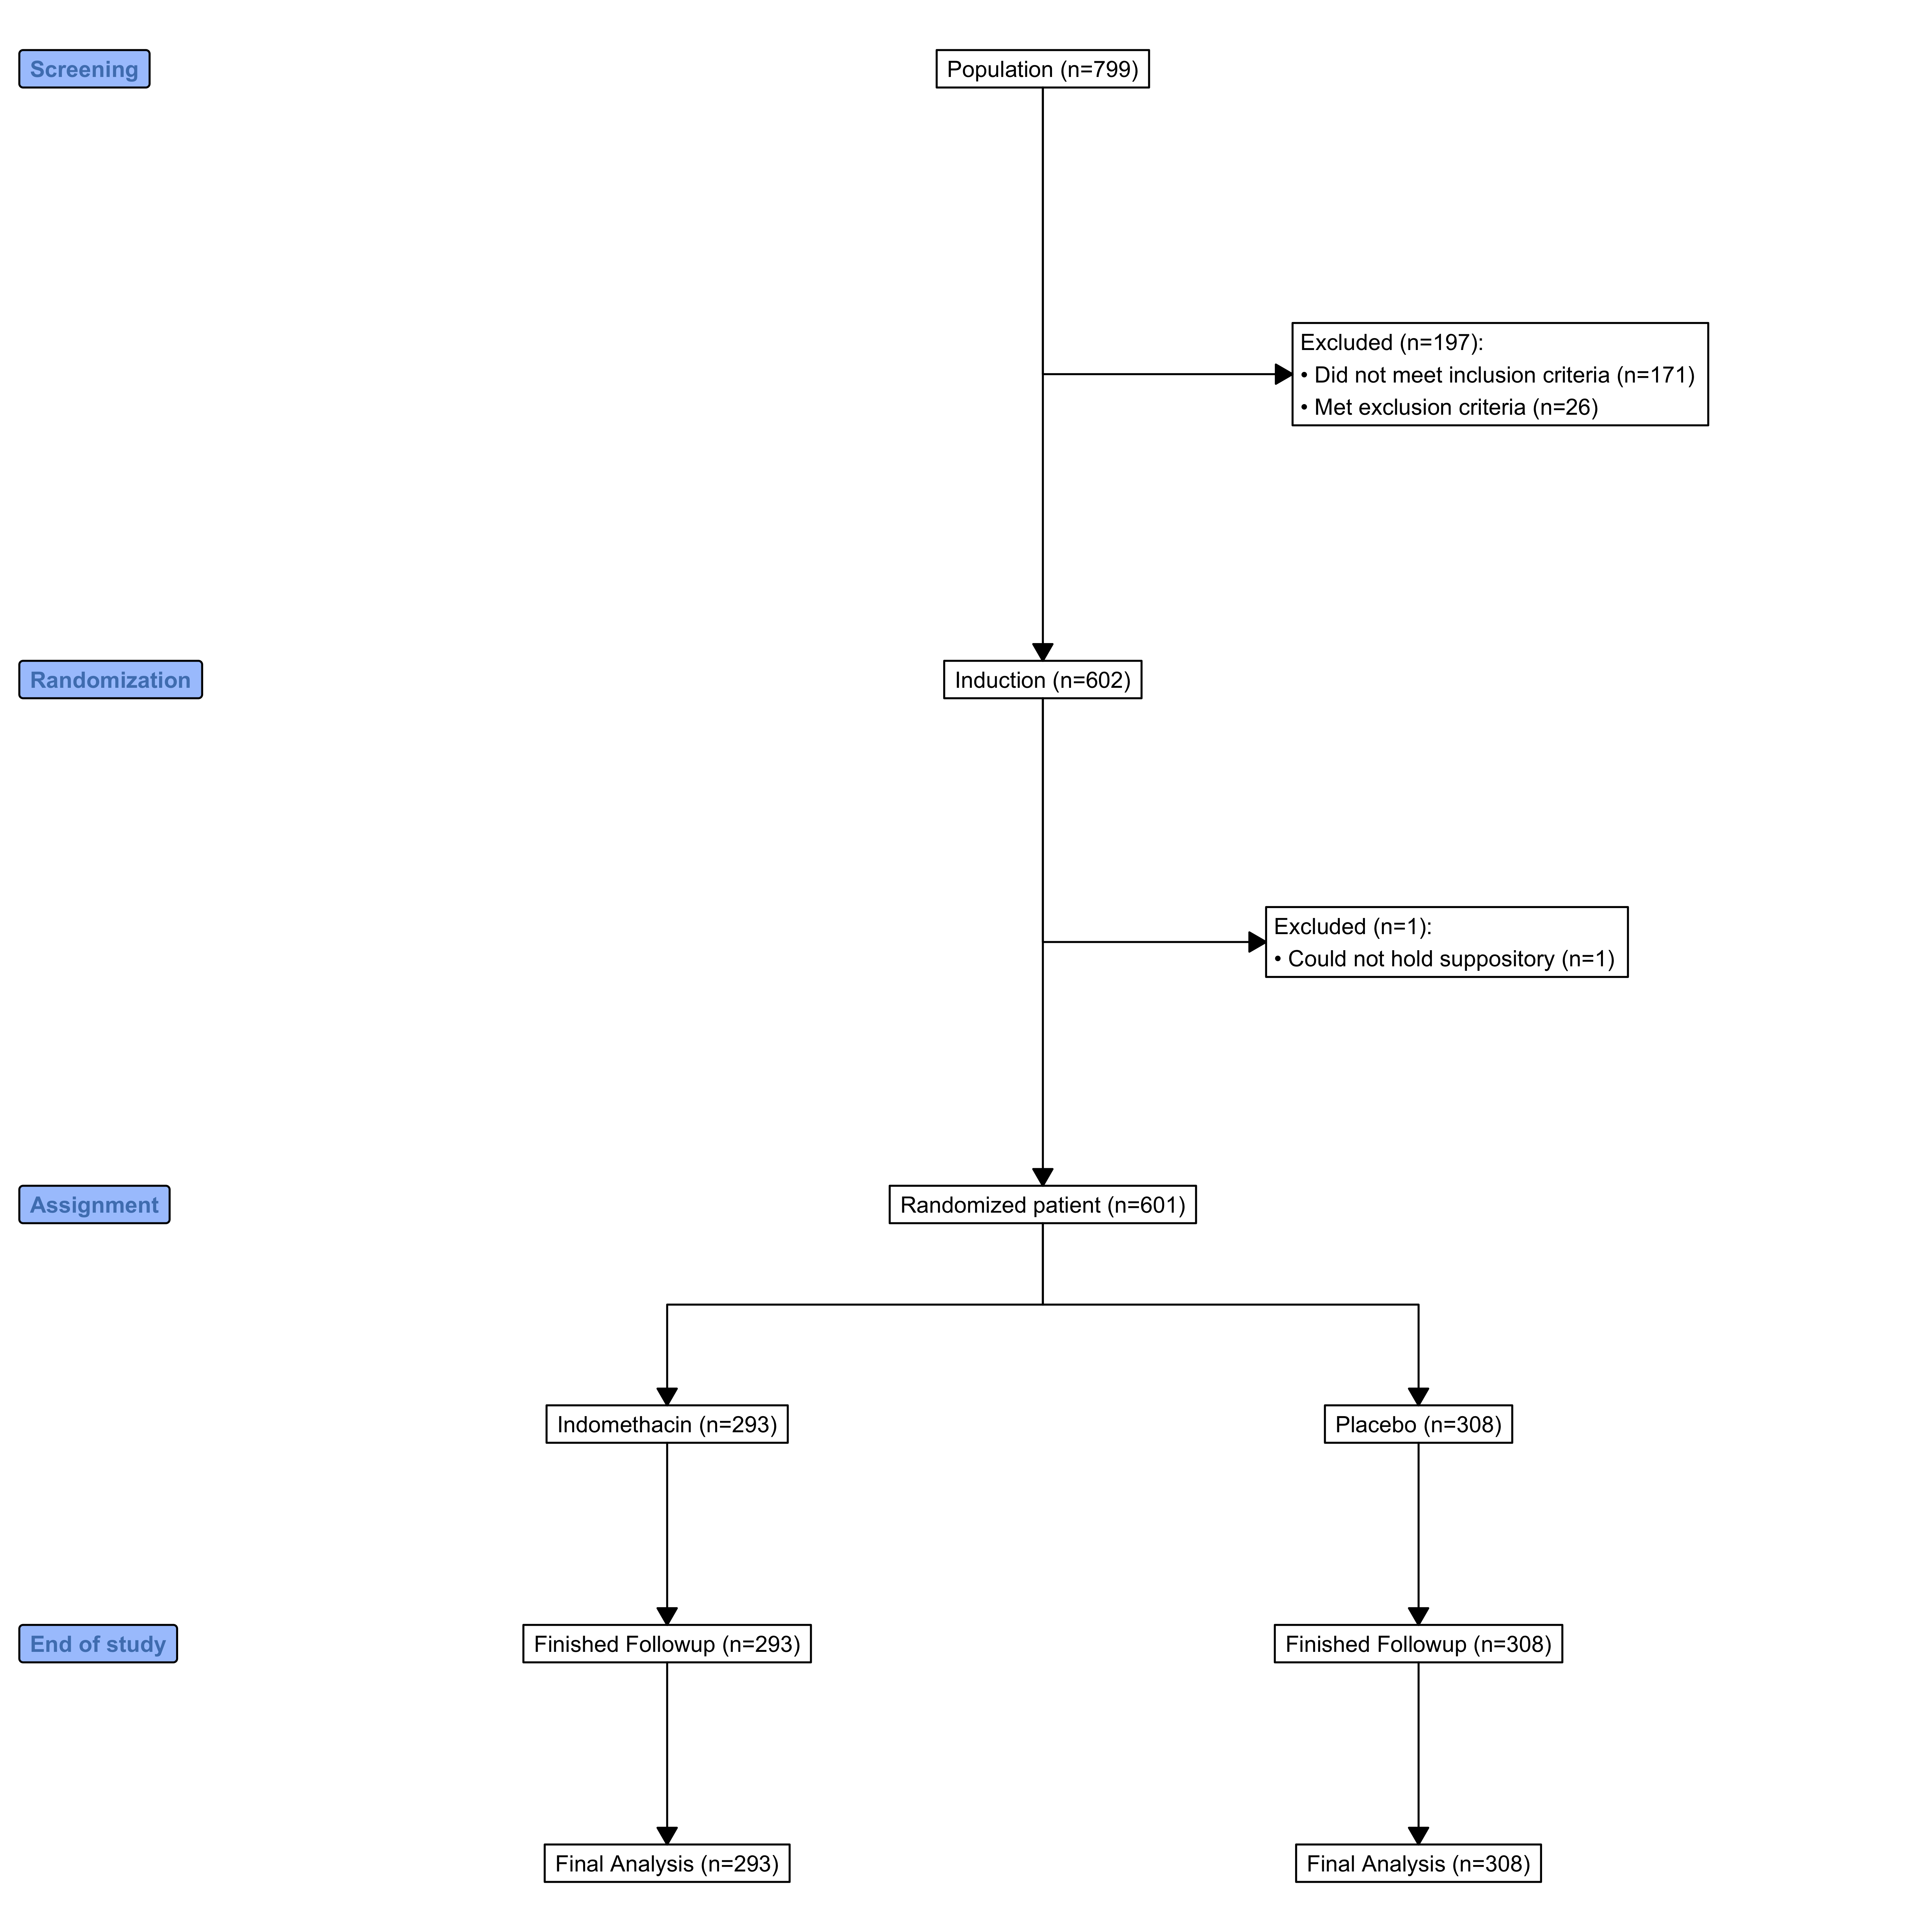
\includegraphics{index_files/figure-latex/notebooks-consort-fig-enrollment-outcomes-output-2.png}

}

\caption{\label{fig-enrollment-outcomes}Enrollment and Outcomes.}

\end{figure}%

\textsubscript{Source:
\href{https://mine-cetinkaya-rundel.github.io/indo-rct/notebooks/consort-preview.html\#cell-fig-enrollment-outcomes}{Enrollment
and Outcomes}}

\textsubscript{Source:
\href{https://mine-cetinkaya-rundel.github.io/indo-rct/index.qmd.html}{Article
Notebook}}

\textsubscript{Source:
\href{https://mine-cetinkaya-rundel.github.io/indo-rct/index.qmd.html}{Article
Notebook}}

A total of 295 patients received indomethacin, and 307 patients received
placebo. One patient in the indomethacin group could not retain the
suppositories but was included in the intention-to-treat analysis.
Follow-up of all patients for the primary and secondary end points was
complete (Fig~\ref{fig-enrollment-outcomes}). Baseline characteristics
were similar in the two study groups
(Table~\ref{tbl-characteristics-baseline}). Notably, 82.2\% of patients
had a clinical suspicion of sphincter of Oddi dysfunction.

\begin{longtable}[]{@{}
  >{\raggedright\arraybackslash}p{(\columnwidth - 8\tabcolsep) * \real{0.1512}}
  >{\centering\arraybackslash}p{(\columnwidth - 8\tabcolsep) * \real{0.0814}}
  >{\centering\arraybackslash}p{(\columnwidth - 8\tabcolsep) * \real{0.2791}}
  >{\centering\arraybackslash}p{(\columnwidth - 8\tabcolsep) * \real{0.3372}}
  >{\centering\arraybackslash}p{(\columnwidth - 8\tabcolsep) * \real{0.1512}}@{}}

\caption{\label{tbl-characteristics-baseline}Characteristics of the
Patients at Baseline.}

\tabularnewline

\toprule\noalign{}
\begin{minipage}[b]{\linewidth}\raggedright
\textbf{Variable}
\end{minipage} & \begin{minipage}[b]{\linewidth}\centering
\textbf{N}
\end{minipage} & \begin{minipage}[b]{\linewidth}\centering
\textbf{0\_placebo}, N = 307
\end{minipage} & \begin{minipage}[b]{\linewidth}\centering
\textbf{1\_indomethacin}, N = 295
\end{minipage} & \begin{minipage}[b]{\linewidth}\centering
\textbf{p-value}
\end{minipage} \\
\midrule\noalign{}
\endhead
\bottomrule\noalign{}
\endlastfoot
\textbf{age} & 602 & 46 (36, 55) & 44 (33, 54) & 0.2 \\
\textbf{gender} & 602 & & & 0.4 \\
1\_female & & 247 (80\%) & 229 (78\%) & \\
2\_male & & 60 (20\%) & 66 (22\%) & \\
\textbf{sod} & 602 & & & 0.2 \\
0\_no & & 60 (20\%) & 47 (16\%) & \\
1\_yes & & 247 (80\%) & 248 (84\%) & \\
\textbf{pep} & 602 & & & \textgreater0.9 \\
0\_no & & 258 (84\%) & 248 (84\%) & \\
1\_yes & & 49 (16\%) & 47 (16\%) & \\
\textbf{recpanc} & 602 & & & 0.7 \\
0\_no & & 213 (69\%) & 209 (71\%) & \\
1\_yes & & 94 (31\%) & 86 (29\%) & \\
\textbf{difcan} & 602 & & & 0.6 \\
0\_no & & 230 (75\%) & 215 (73\%) & \\
1\_yes & & 77 (25\%) & 80 (27\%) & \\
\textbf{precut} & 602 & & & 0.8 \\
0\_no & & 290 (94\%) & 280 (95\%) & \\
1\_yes & & 17 (5.5\%) & 15 (5.1\%) & \\
\textbf{paninj} & 602 & & & 0.2 \\
0\_no & & 271 (88\%) & 270 (92\%) & \\
1\_yes & & 36 (12\%) & 25 (8.5\%) & \\
\textbf{psphinc} & 602 & & & 0.4 \\
0\_no & & 137 (45\%) & 122 (41\%) & \\
1\_yes & & 170 (55\%) & 173 (59\%) & \\
\textbf{acinar} & 602 & & & 0.5 \\
0\_no & & 295 (96\%) & 280 (95\%) & \\
1\_yes & & 12 (3.9\%) & 15 (5.1\%) & \\
\textbf{bsphinc} & 602 & & & 0.5 \\
0\_no & & 136 (44\%) & 122 (41\%) & \\
1\_yes & & 171 (56\%) & 173 (59\%) & \\
\textbf{amp} & 602 & & & \textgreater0.9 \\
0\_no & & 298 (97\%) & 286 (97\%) & \\
1\_yes & & 9 (2.9\%) & 9 (3.1\%) & \\
\textbf{pdstent} & 602 & & & 0.4 \\
0\_no & & 58 (19\%) & 48 (16\%) & \\
1\_yes & & 249 (81\%) & 247 (84\%) & \\
\textbf{train} & 602 & & & 0.5 \\
0\_no & & 167 (54\%) & 152 (52\%) & \\
1\_yes & & 140 (46\%) & 143 (48\%) & \\

\end{longtable}

\textsubscript{Source:
\href{https://mine-cetinkaya-rundel.github.io/indo-rct/index.qmd.html}{Article
Notebook}}

\subsection{Study outcomes}\label{study-outcomes}

The primary outcome of post-ERCP pancreatitis occurred in 79 of 602
patients (13.1\%). Of these events, 27 of 295 (9.2\%) occurred in the
indomethacin group and 52 of 307 (16.9\%) occurred in the placebo group
(P=0.005), corresponding to an absolute risk reduction of 7.7 percentage
points (number needed to treat {[}NNT{]} to prevent one episode of
post-ERCP pancreatitis, 13) and a relative risk reduction of 46\%
(Fig~\ref{fig-incidences-adverse-events}).

\begin{figure}[H]

\centering{

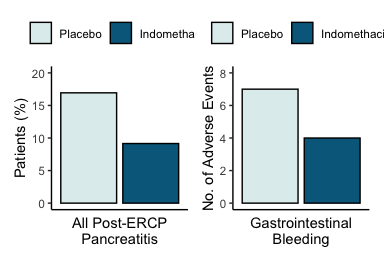
\includegraphics{index_files/figure-latex/notebooks-incidences-fig-incidences-adverse-events-output-1.png}

}

\caption{\label{fig-incidences-adverse-events}Incidence of the Primary
and Secondary End Points and Adverse Events}

\end{figure}%

\textsubscript{Source:
\href{https://mine-cetinkaya-rundel.github.io/indo-rct/notebooks/incidences-preview.html\#cell-fig-incidences-adverse-events}{Incidence
of the Primary and Secondary End Points and Adverse Events}}

All 79 patients with post-ERCP pancreatitis completed the 30-day
follow-up necessary to determine the severity of post-ERCP pancreatitis.
The secondary outcome of moderate or severe post-ERCP pancreatitis
occurred in 40 patients: 13 (4.4\%) in the indomethacin group and 27
(8.8\%) in the placebo group (P=0.03)
(Fig~\ref{fig-incidences-adverse-events}). Three patients in each group
had severe post-ERCP pancreatitis, and one patient in the placebo group
had pancreatic necrosis.

Among patients with post-ERCP pancreatitis, the median length of
hospital stay was 0.5 days shorter in the indomethacin group than in the
placebo group (3.5 vs.~4.0 days, P\textless0.001).

\subsubsection{Heterogeneity in Treatment
Effects}\label{heterogeneity-in-treatment-effects}

The relative benefit of indomethacin did not vary significantly
according to patients' pretreatment risk score, although the absolute
risk reduction varied from an NNT of 21 for those with a risk score of 1
(one major or two minor inclusion criteria) to an NNT of 6 for those
with a risk score of 5 (e.g., four major and two minor inclusion
criteria) (Fig~\ref{fig-heterogeneity}).

\begin{figure}

\centering{

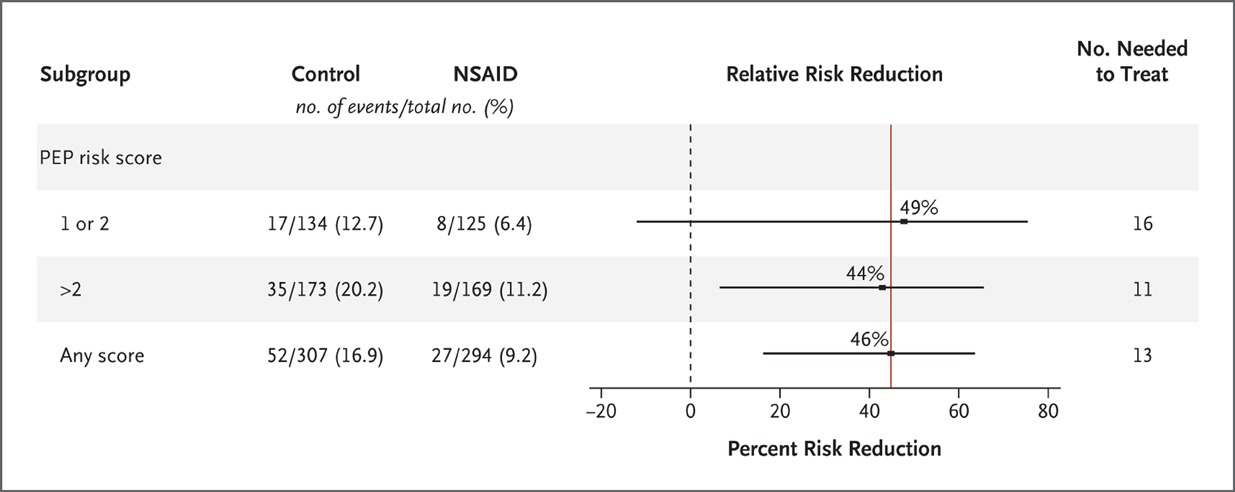
\includegraphics{images/clipboard-2828008318.png}

}

\caption{\label{fig-heterogeneity}Analysis of the Heterogeneity in
Treatment Effects.}

\end{figure}%

\subsection{Exploratory Subgroup
Analyses}\label{exploratory-subgroup-analyses}

The beneficial effect of indomethacin on the primary outcome was also
consistent across the other prespecified and post hoc secondary
subgroups (Fig~\ref{fig-exploratory-subgroup}). In particular,
indomethacin appeared to be protective regardless of whether patients
had undergone pancreatic stenting or had a clinical suspicion of
sphincter of Oddi dysfunction; indomethacin was also protective in all
three subtypes of sphincter of Oddi dysfunction and in the two study
sites enrolling the largest number of patients.

\begin{figure}

\centering{

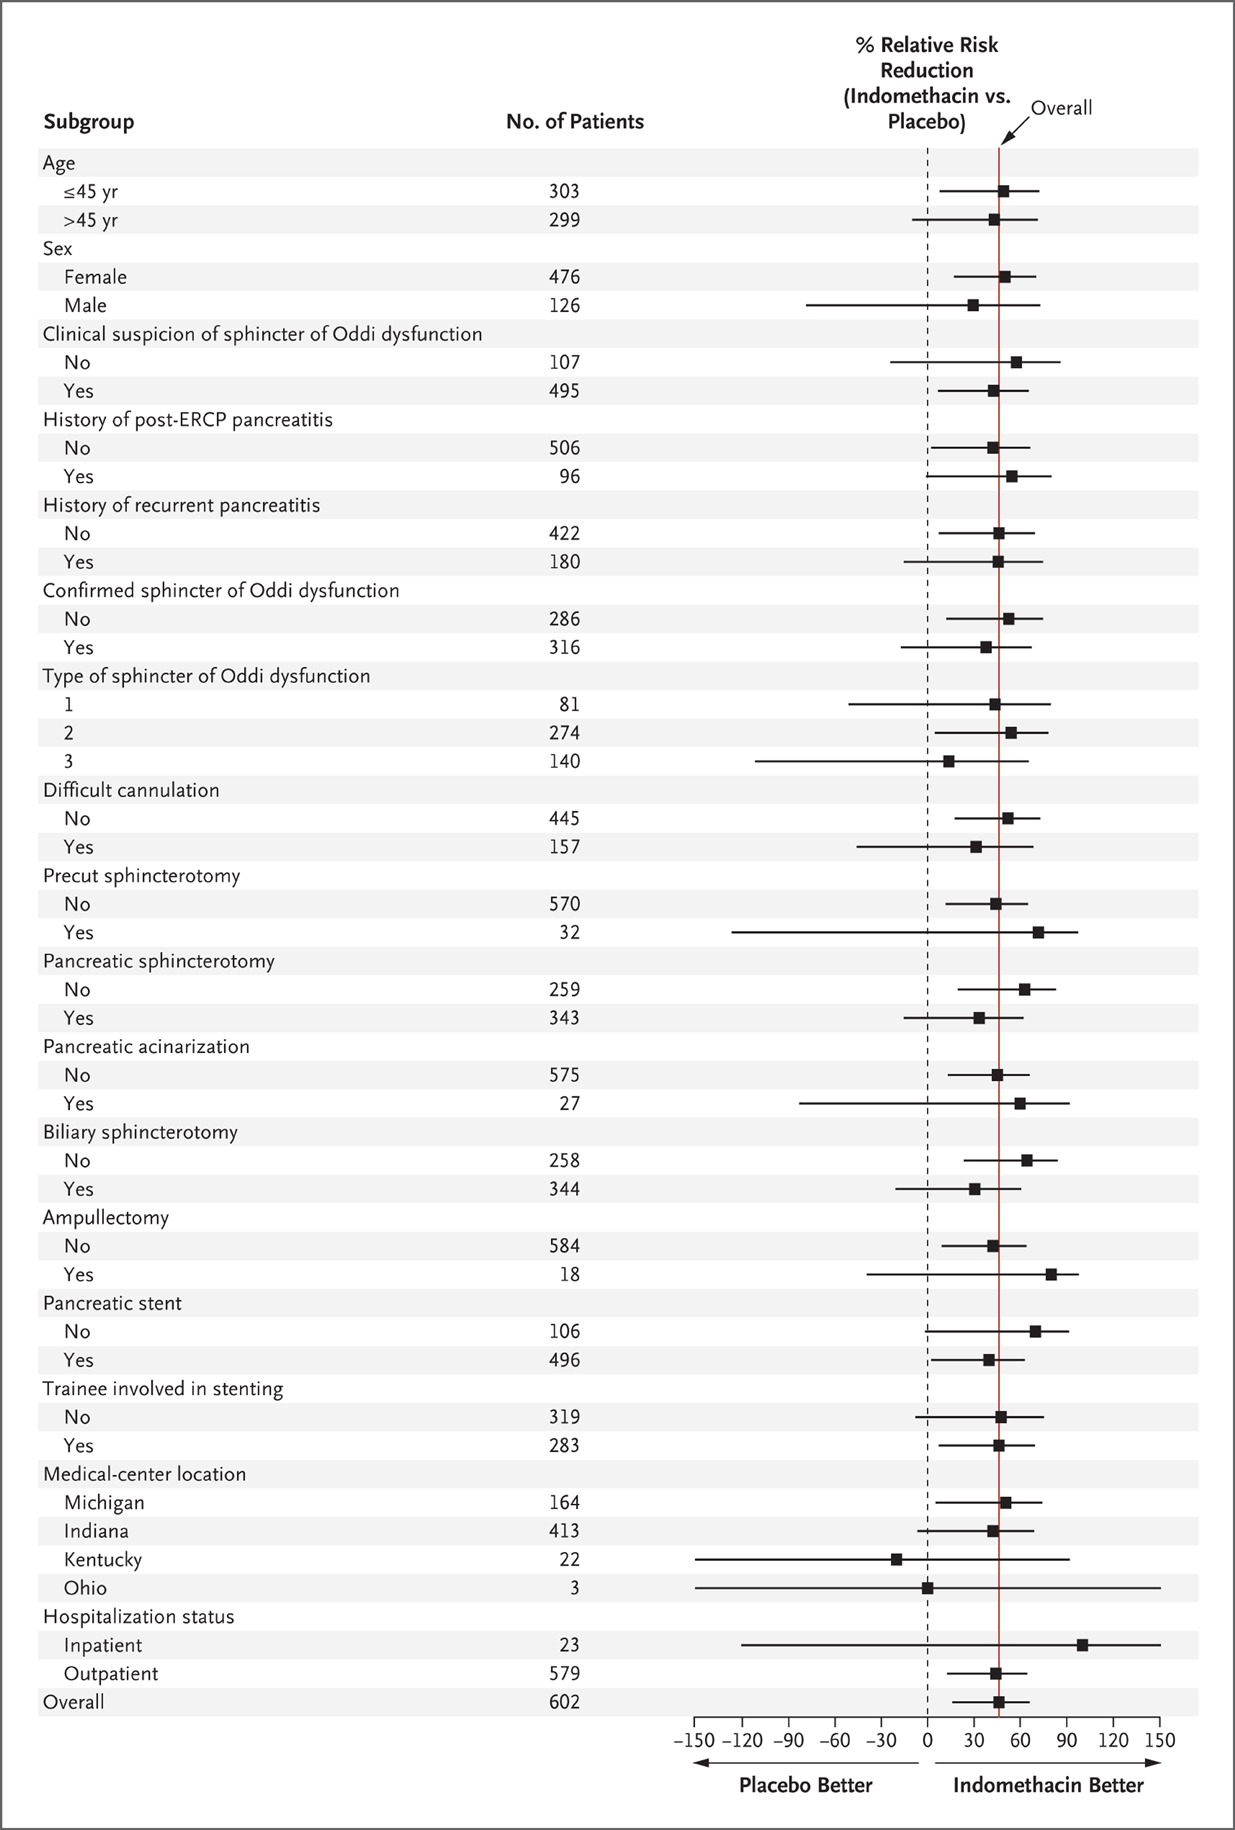
\includegraphics{images/clipboard-1822931444.png}

}

\caption{\label{fig-exploratory-subgroup}Exploratory Subgroup Analyses}

\end{figure}%

\subsection{Adverse Events}\label{adverse-events-1}

There were 13 adverse events that were potentially attributable to the
study intervention (Fig~\ref{fig-incidences-adverse-events}). Clinically
significant bleeding occurred in 11 patients (1.8\%): 4 in the
indomethacin group and 7 in the placebo group (P=0.72). None of the
bleeding events resulted in transfusion of more than 2 units of packed
red cells or required angiography or surgery for treatment. Two cases of
acute renal failure occurred, both in the placebo group. There were no
myocardial infarctions, strokes, or deaths at 30-day follow-up.

\section{Discussion}\label{discussion}

Our findings showed that one dose of rectal indomethacin given
immediately after ERCP significantly reduced the incidence of post-ERCP
pancreatitis in patients at elevated risk for this complication.
Moreover, we found that prophylactic indomethacin decreased the severity
of post-ERCP pancreatitis and was associated with a shorter hospital
stay. In this trial, the number of high-risk ERCP patients who would
need to be treated to prevent one episode of pancreatitis was 13.

The majority of patients in this study had a clinical suspicion of
sphincter of Oddi dysfunction, and more than half had sphincter
hypertension, as documented on manometry, which suggests that the
results are particularly applicable to this challenging patient
population. However, among patients who received indomethacin, there was
a trend toward benefit with respect to rates of post-ERCP pancreatitis
for those who did not have a clinical suspicion of sphincter of Oddi
dysfunction (8.5\% vs.~20.0\%, P=0.11). Moreover, in a subgroup
analysis, the relative treatment effect of indomethacin was consistent
across the spectrum of patients' risk of post-ERCP pancreatitis.
Additional studies will be necessary to reproduce our results in
different patient populations and to determine whether indomethacin is
effective in low-risk patients, as suggested by our previous
meta-analysis.\citep{andriulli2007}

Although more than 80\% of the patients in this clinical trial underwent
pancreatic stenting on the basis of their elevated risk of post-ERCP
pancreatitis, certain patients did not receive stents, either because
the endoscopist did not deem it indicated (e.g., difficult cannulation
not requiring a precut sphincterotomy) or because placement was not
technically feasible (failed pancreatic access). Among patients who
received a pancreatic stent, indomethacin reduced the risk of post-ERCP
pancreatitis from 16.1\% to 9.7\% (P=0.04). Indomethacin conferred
similar benefit in patients who did not receive a pancreatic stent,
reducing the risk of post-ERCP pancreatitis from 20.6\% to 6.3\%
(P=0.049).

Congruent with previous clinical trials evaluating NSAIDs in the
prevention of post-ERCP pancreatitis, the risk of adverse events that
were potentially attributable to indomethacin in this study was similar
in the two study groups. Specifically, there was no significant
between-group difference in the frequency or severity of bleeding
events. This finding is consistent with previously published data
suggesting that NSAIDs in standard doses do not increase the risk of
bleeding after biliary
sphincterotomy.\citep{freeman1996, nelson1994major} Of note, patients
with contraindications to NSAIDs, such as renal failure and active
peptic-ulcer disease, were excluded from this study.

The rate of post-ERCP pancreatitis in the placebo group (16.9\%)
exceeded that revealed by the internal audit of high-risk ERCP patients
at participating institutions (16.9\% vs.~10\%). (These audit results
had been used to calculate the sample size.) This difference may be due
to the increased capture of complications that occurs in randomized,
controlled trials. Nevertheless, the incidence of post-ERCP pancreatitis
in the placebo group of this trial was similar to that in previous
studies of NSAID pharmacoprevention in high-risk subjects, in which the
mean rate of post-ERCP pancreatitis was 18.8\%.\citep{andriulli2007}

In summary, prophylactic rectal indomethacin significantly reduced the
incidence and severity of post-ERCP pancreatitis in patients at elevated
risk for this complication, particularly in those with a clinical
suspicion of sphincter of Oddi dysfunction.


\nolinenumbers
  \bibliography{references.bib}

\end{document}
